\chapter{Analys av punktmolnsregistrering}
\label{cha:indiv-report-karlsson}
\chapterprecis{\LARGE{---- Michael Karlsson ----}}


\section{Inledning}
\label{sec:introduction-karlsson}

%% Skriv här
I denna rapport behandlas undersökningen av olika registreringsalgoritmer utförd av Michael Karlsson i samband med TDDD96 \textit{Kandidatprojekt i programvaruutveckling} samt de problem som projektgruppen stött på gällande registrering av punktmoln.

\subsection{Syfte}
\label{sec:purpose-karlsson}

Syftet med den här delen är att väga olika algoritmer mot varandra och undersöka hur väl de fungerade för det projekt som beskrivs i övriga rapporten samt vilka problem gruppen hade med de olika algoritmer som testades. Gruppens tillvägagångssätt för val av algoritm undersöks också.


\subsection{Frågeställningar}
\label{sec:issue-karlsson}

\begin{enumerate}
	\item Hur skapas ett enhetligt punktmoln från bilder tagna med en fast avståndskamera?
	\item Hur gör man för att välja algoritm och hur resonerade gruppen när de valde ICP?	
\end{enumerate}

\subsection{Definitioner och förkortningar}
\label{sec:definitions-acronyms-karlsson}

Här listas de definitioner och förkortningar som används i den här delen av rapporten.

\begin{itemize}
	\item Point Cloud Library (PCL) \cite{pcl_home} - Ett C++ bibliotek för hantering av punktmoln.
	\item Iterative Closest Point (ICP) - En algoritm för punktmolnsregistrering.
	\item JR-MPC \cite{Evangelidis-ECCV-2014} - Joint Registration of Multiple Point Clouds.
\end{itemize}


\subsection{Avgränsningar}
\label{sec:limits-karlsson}
För registrering finns en ofantlig mängd algoritmer och tillvägagångssätt. Denna utredning begränsas till de metoder som använts inom projektet. 


\section{Bakgrund}
\label{sec:background-karlsson}
I ett tidigt stadie av projektet upptäckte gruppen att en stor del skulle handla om att få registrering av punktmoln att fungera bra. Tidiga tester visade dessutom att meshningen, en annan del som tidigt verkade omfattande, som görs efter registreringen var förhållandevis enkel att utföra. Meshning innebär att det, utifrån det kompletta punktmolnet, skapas en vattentät 3D-modell. Författaren blev intresserad efter att ha jobbat  med tidiga försök till registrering och påbörjade en djupdykning i ämnet.


\section{Teori}
\label{sec:theory-karlsson}

För att återskapa fysiska objekt digitalt saknas lämpliga verktyg, såsom tex en 3D-kamera. Istället behöver flera bilder av objektet tas från olika vinklar för att kunna sammanfoga dessa till det kompletta objektet. Det finns många metoder för detta, exempelvis Kinect Fusion, se avsnitt \ref{sec:kinect-karlsson}. Den metod projektgruppen använt sig av har dock bestått av en avståndskamera på en linjärenhet med objektet monterat på ett rotationsbord med två rotationsaxlar. Med hjälp av detta rotationsbord kan hela objektet ses från en fast punkt. Det primära målet har varit att enhetligt registrera de punktmoln som kommit av skanningar med denna uppställning till en komplett representation av objektet.


\subsection{Registrering}
\label{sec:registrering-karlsson}

Registrering är den generella metoden att sätta ihop två eller flera punktmoln till ett i ett gemensamt koordinatsystem med all information från punktmolnen. Det finns väldigt många olika algoritmer för att utföra detta såsom till exempel ICP, eller GMMReg, \textit{Gaussian Mixture Model Registration}. De flesta tillgängliga algoritmer har någon form av svaghet eller nackdel. Till exempel lider ICP av så kallad \textit{felutbredning}, där ett litet fel i ett stadie orsakar större fel i senare stadier och JR-MPC, som utnyttjar GMM, lider av längre körtid \cite{Evangelidis-ECCV-2014}.

\subsection{Kinect Fusion}
\label{sec:kinect-karlsson}
Kinect Fusion använder sig av Microsofts egna avstånds- och RGB-kamera, Kinect, för att mappa upp ett 3D-objekt i den verkliga världen. Avståndskameran mäter upp punktmolnet för scenen framför den samtidigt som en synkroniserad RGB-kamera ger färgdata till varje punkt. 
Varje punktmoln som Kinect-kameran skickar består av ca. 307 000 punkter. Det kan jämföras med hårdvaran som använts av gruppen där maximala antalet punkter i en skanning är ca. 786 000 punkter. De punktmoln som använts har dock generellt innehållit ca 30-60\,000 punkter efter filtrering av skräpdata. Skräpdata är de punkter som inte är intressanta. Registreringen som görs av Kinect Fusion är en variant av ICP.

\section{Metod}
\label{sec:method-karlsson}

Här presenteras metoden som använts för att besvara frågeställningarna i den här rapporten. De är uppdelade i hur arbetet för att besvara frågorna gick till i förstudien samt under utvecklingsarbetet för rapporten.

\subsection{Litteraturstudie}
Initialt gjordes en litteraturstudie för att hitta information om vilka tillvägagångssätt för att registrera punktmoln som finns. De söktermer som använts är "registration pointcloud" samt "registration algorithm". Sökmotorn som använts är Google Scholar. De källor som undersökts har begränsats till att vara relaterade till JR-MPC samt ICP.

\subsection{Experiment}
Ett experiment utfördes för att jämföra ICP och JR-MPC. Experimentet gick ut på att registrera en uppsättning av 36 punktmoln. Vart och ett av dessa punktmoln var en skanning av kyrkan, se figur \ref{fig:karlsson-single_scan-church}, där kyrkan skannats och roterats 10 grader efter varje skanning. 3DCopy användes för att testa ICP medan JR-MPC testades med kod som tillhandahålls av skaparna, skriven i MatLab. För JR-MPC är enbart inläsningen av indata modifierad. För ICP valdes \textit{Max Correspondence Distance} till 15, \textit{Max Iterations} sattes till 100 samt \textit{Transformation Epsilon} var satt till $ 1e-8 $. Övriga parametrar i PCLs implementation av ICP användes utan modifikation. För beskrivning av dessa parametrar, se avsnitt \ref{sec:icp-karlsson}. Varje algoritm kördes tre gånger och resultatet mellan körningarna jämfördes. Testdatan finns tillgänglig på GitHub \cite{mickwald_testdata}. PCD-filerna användes för 3DCopy medan TXT-filerna användes för JR-MPC. TXT-filerna skapades genom att kopiera PCD-filerna, byta filändelse samt ta bort den \textit{header} som finns i PCD-filerna. Punkterna i TXT-filen är därmed identiska med PCD-filerna.

\begin{figure}[H]
	\centering
	\includegraphics[width=50mm]{figures/Foto_church.png}
	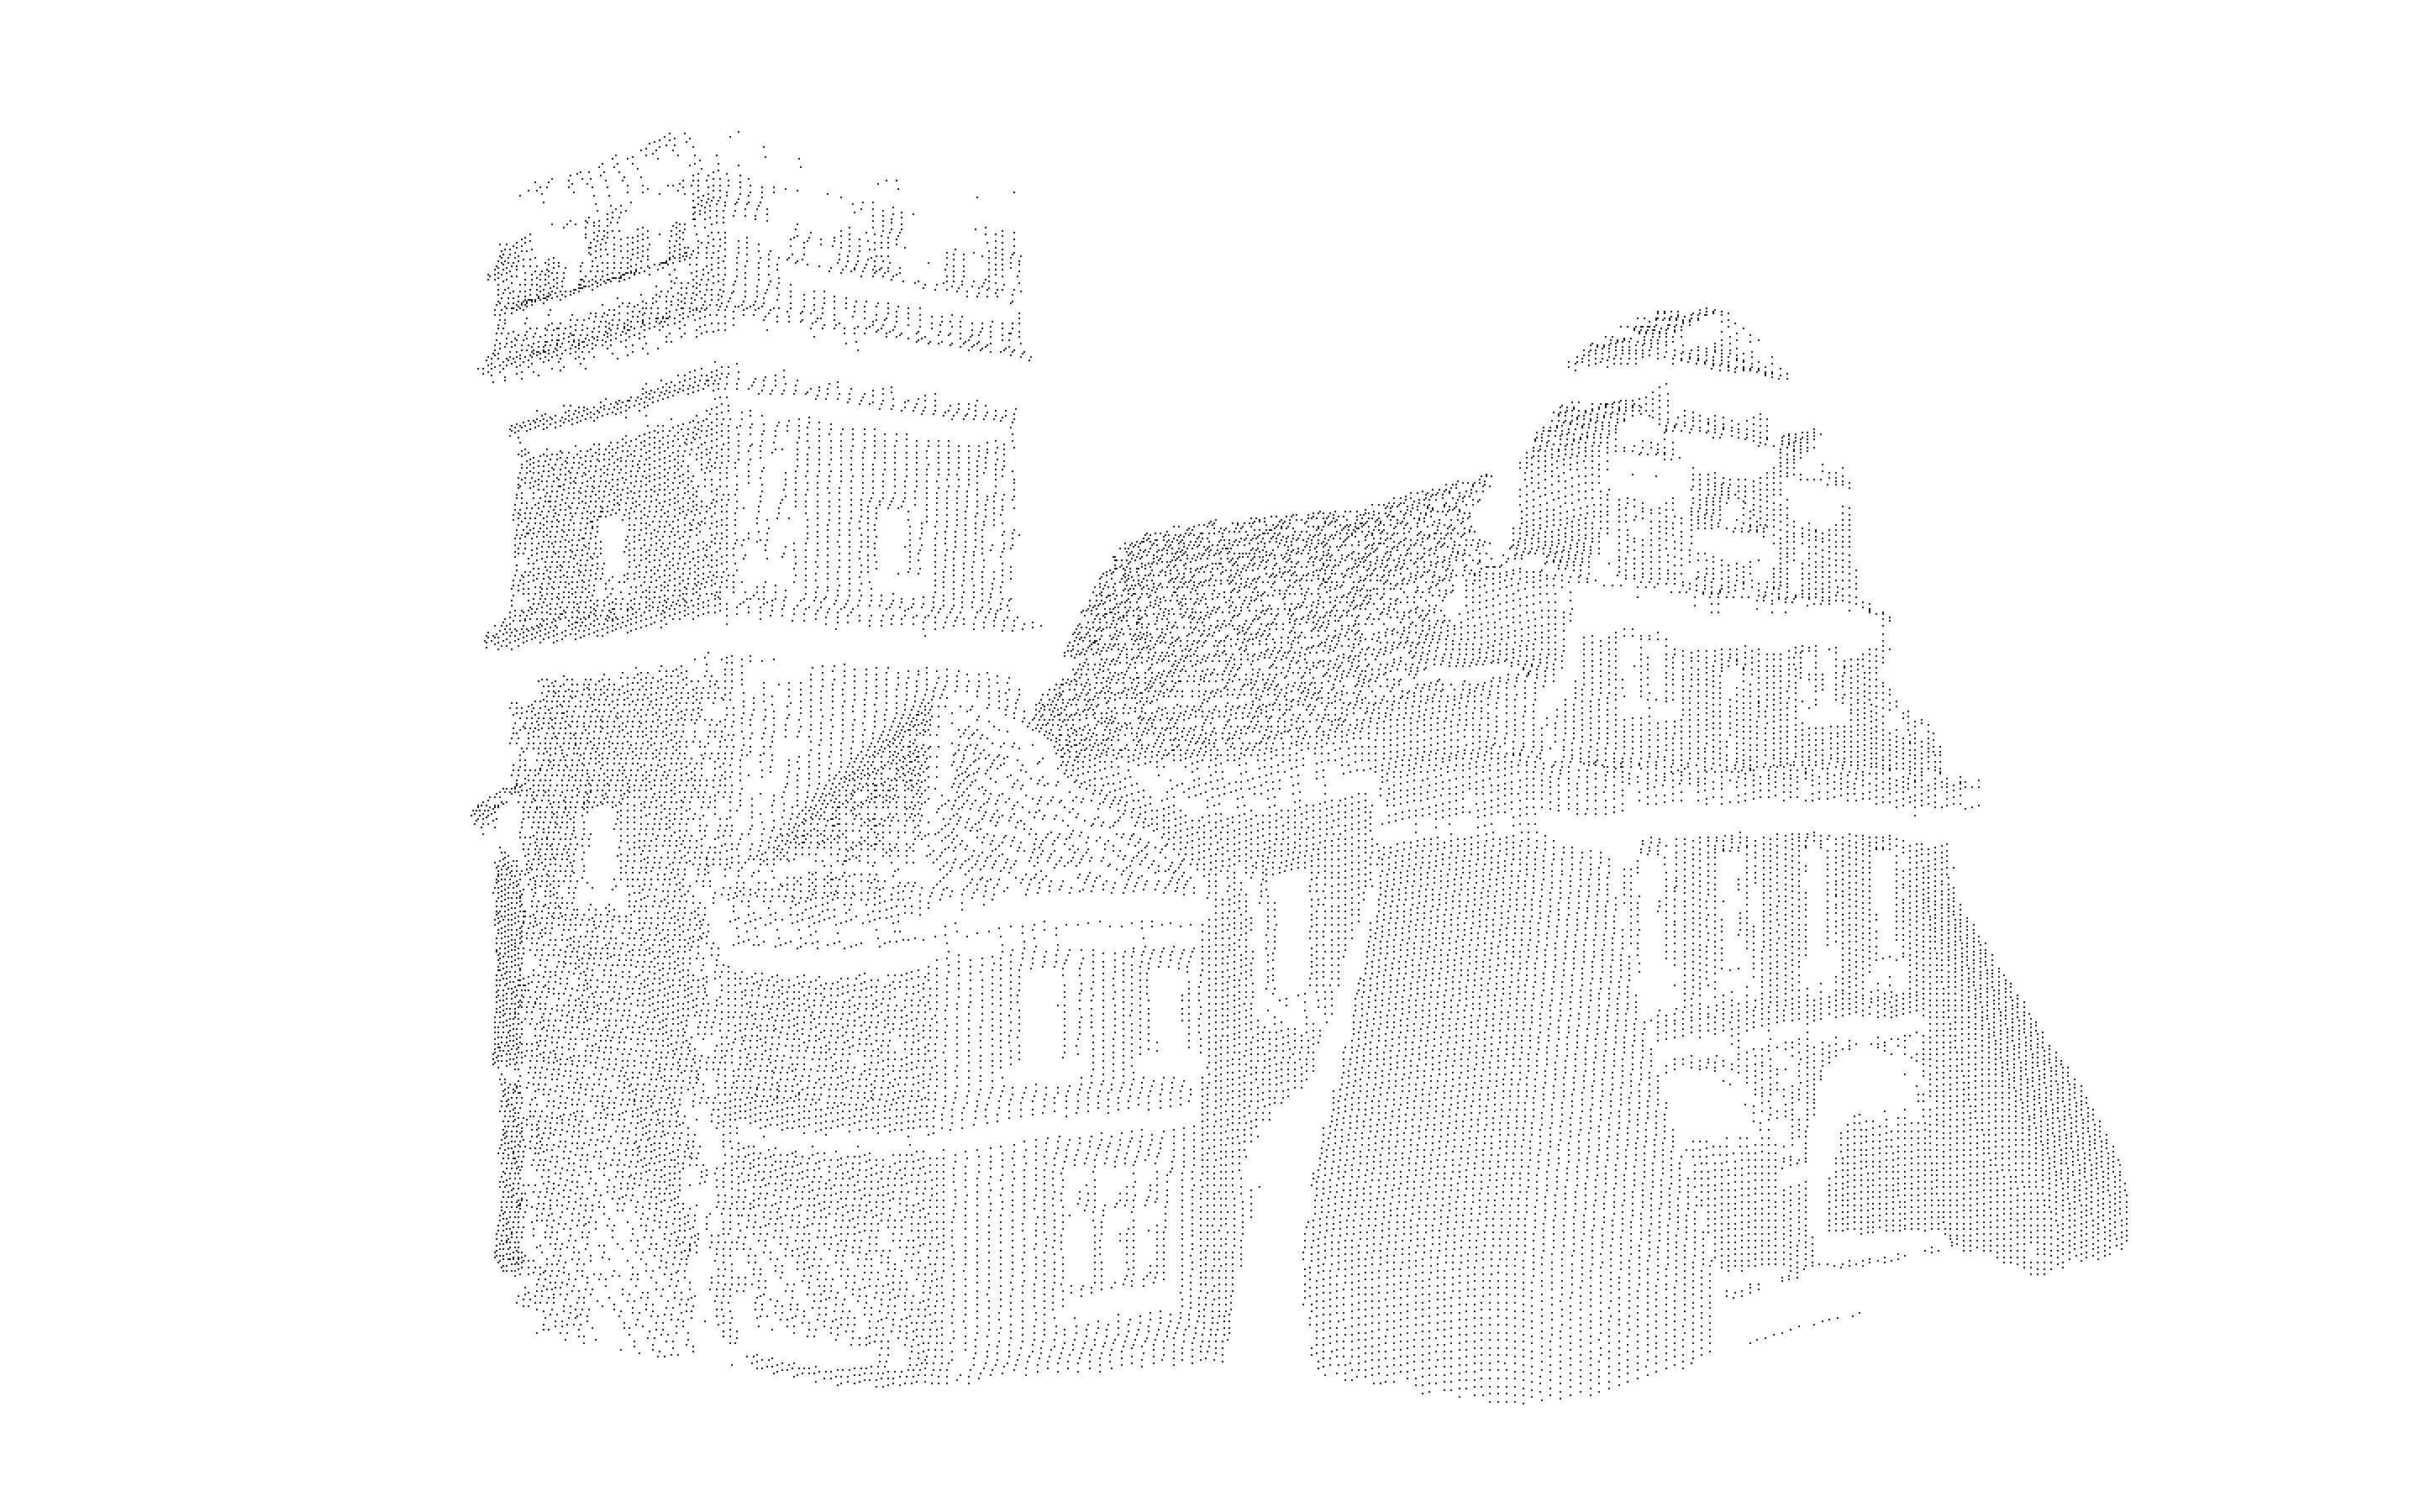
\includegraphics[width=90mm]{figures/icke_komplett_moln_kyrka.png}
	\caption{Kyrkan som skannats samt ett resulterande punktmoln från en enkel skanning.}
	\label{fig:karlsson-single_scan-church}
\end{figure}


\section{Resultat}
\label{sec:results-karlsson}

Här presenteras av resultatet av den litteraturstudie som genomförts samt den jämförelse som gjorts baserat på studien. Dessutom presenteras resultatet av det experiment som utförts.

\subsection{Litteraturstudie}
PCL \cite{pcl_home} ger många handledningsexempel med exempelkod som var utgångspunkten för gruppens registreringsalgoritm. PCL ger också en bra sammanfattning men utöver det saknas relevanta källor. Då utredningen är begränsad till ICP och JR-MPC begränsas antalet källor ytterligare. Det finns enormt många varianter av ICP, såsom SequentialICP, Point-to-Plane ICP, Point-to-Point ICP m.fl. Den variant som utvärderas här är den som implementeras av PCL, Point-to-Point. 

JR-MPC \cite{Evangelidis-ECCV-2014} är resultatet av en forskningsstudie som tagit fram algoritmen och därmed finns enbart den källa som används här för den algoritmen.

Bellekens et al. \cite{beller2014modern} presenterar en genomgående studie där olika algoritmer jämförs. 

\subsubsection{ICP}
\label{sec:icp-karlsson}
ICP är en optimeringsalgoritm som försöker minimera det totala avståndet från varje punkt i ursprungsmolnet till varje punkt i målmolnet. Det ger algoritmen en tidskomplexitet $ \mathit{O(n*m)} $ där $ \mathit{n} $ är antalet punkter i ursprungsmolnet och $ \mathit{m} $ är antalet punkter i målmolnet. ICP ett ursprungsmoln som aldrig ändras samt ett målmoln som algoritmen försöker passa in så att det stämmer överens med ursprungsmolnet. 

ICP har ett antal parametrar för att bestämma hur registreringen ska gå till. De parametrar som undersökts inom gruppen beskrivs nedan.
\begin{itemize}
	\item \textbf{Max Iterations} anger hur många registrerings\-iterationer som algoritmen får utföra innan den tvingas avsluta.
	\item \textbf{Transformation Epsilon} avgör hur stor förflyttning algoritmen får göra på målmolnet inom en iteration.
	\item \textbf{Max Correspondence Distance} anger hur stort avståndet från en punkt i ursprungsmolnet till motsvarande punkt i målmolnet får vara. Är avståndet större än detta kommer algoritmen ignorera punkten i målmolnet vid registreringsförsöket.
	\item \textbf{RANSAC Outlier Rejection Threshold} anger hur stort avstånd som en punkt tillåts existera från den antagna matematiska modellen för att användas i registreringen. RANSAC, \textit{Random Sample Consensus} är en metod för att avgöra om en punkt följer det matematiska mönster som algoritmen letar efter.
	\item \textbf{Euclidean Fitness Epsilon} representerar det fel som accepteras. Är skillnaden i felet mellan två iterationer mindre än det här kommer algoritmen avsluta.
\end{itemize}

\subsubsection{JR-MPC}
JR-MPC använder en så kallade GMM, \textit{Gaussian Mixture Model}, för att registrera objektet. Exakt hur matematiken bakom algoritmen ser ut och fungerar är utanför omfattningen av denna rapport men grundläggande principer följer. GMM är en sannolikhetsmodell som används för att lista sannolikheten att ett kluster av punkter i punktmolnet är en del av objektet som ska registreras, detta motsvarar RANSAC filtreringen som görs i ICP. Själva registreringen görs genom en villkorlig maximering, ECM, \textit{Expectation Conditional Maximization} som optimerar registreringen med begränsade variationer i registreringsparameterar. För fördjupning om ECM hänvisas till Roche \cite{roche2011algorithm}.

\subsection{ICP vs. JR-MPC}

Vid jämförande av ICP och JR-MPC finns ett par signifikanta skillnader. Dessa presenteras här.

På grund av att ICP är en mer rudimentär algoritm än JR-MPC blir den också lättare att implementera. JR-MPC bygger på mer avancerad matematik som måste förstås för att kunna implementera den.

Enligt Evangelidis et al. \cite{Evangelidis-ECCV-2014} är ICP en aning snabbare än JR-MPC vilket dock inte har replikerats i projektets begränsade tester. Då tidsåtgången för komplett registrering av 36 punktmoln med ICP är i närheten av tre timmar har inte någon ingående studie genomförts. 

Som nämndes i avsnitt \ref{sec:registrering-karlsson} påverkas algoritmerna väldigt olika av fel, såsom till exempel avrundningsfel som är oundvikligt med flyttal. Då ICP\footnote{Notera att detta endast gäller vissa ICP algoritmer} bara tillåter parvis registrering, det vill säga att ett punktmoln registreras med ett annat kommer dessa avrundningsfel växa och bli större ju fler punktmoln som registreras. Dessutom sparas i 3DCopy det parvis registrerade punktmolnet som ett färdigt oföränderligt punktmoln och ev avrundningsfel kan bara elimineras genom att köra algoritmen igen med andra parametrar.

\subsection{Experiment}

Resultatet av experimentet som utfördes presenteras här med hjälp av ett antal bilder.  

\begin{figure}[H]
	\centering
	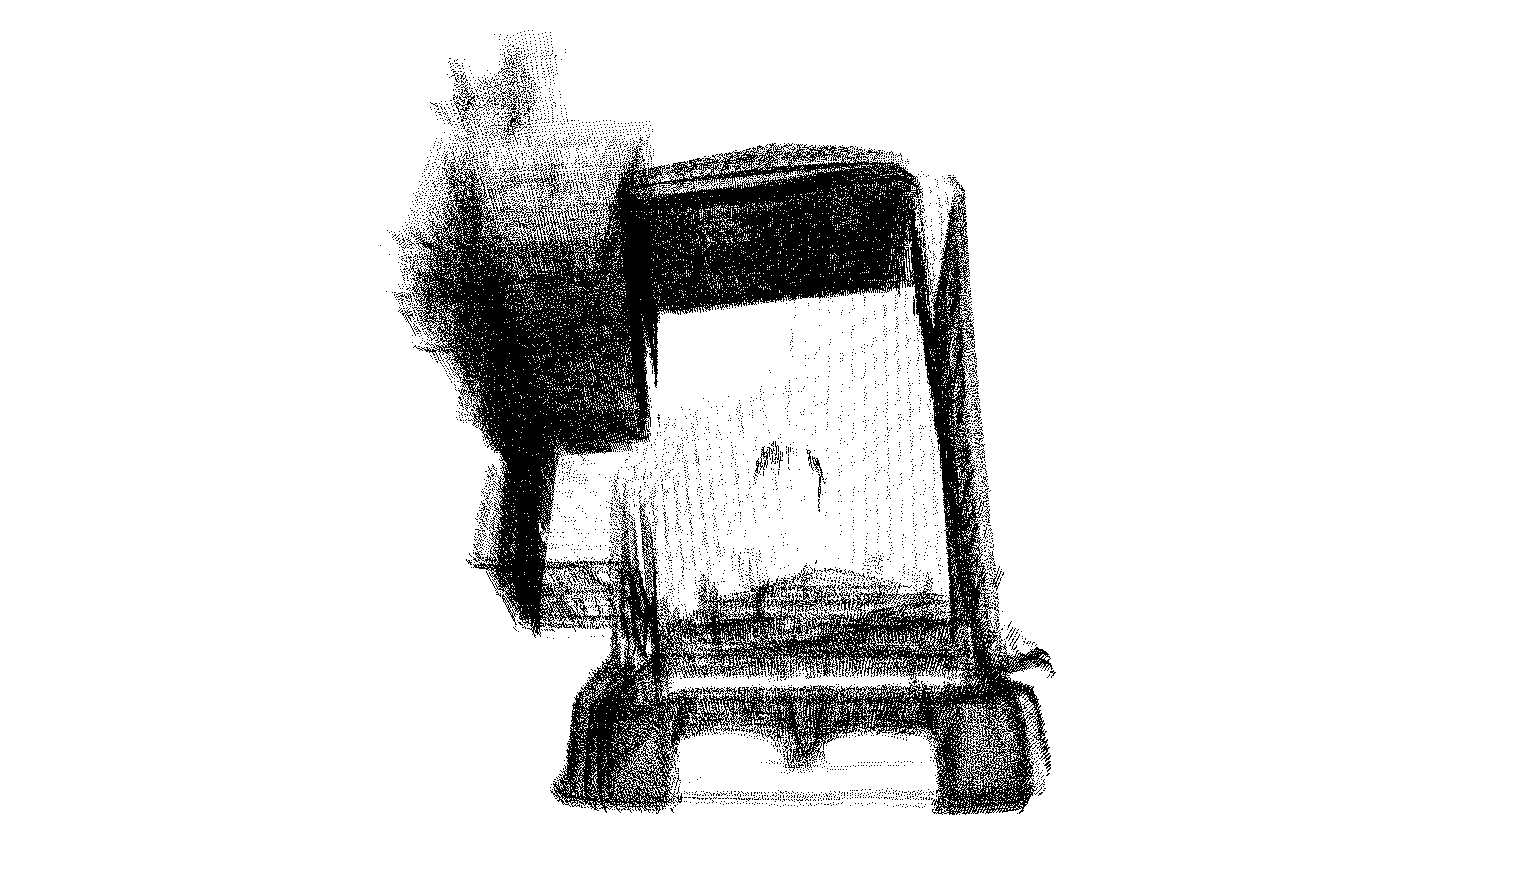
\includegraphics[width=65mm]{figures/first_registered_church.png}
	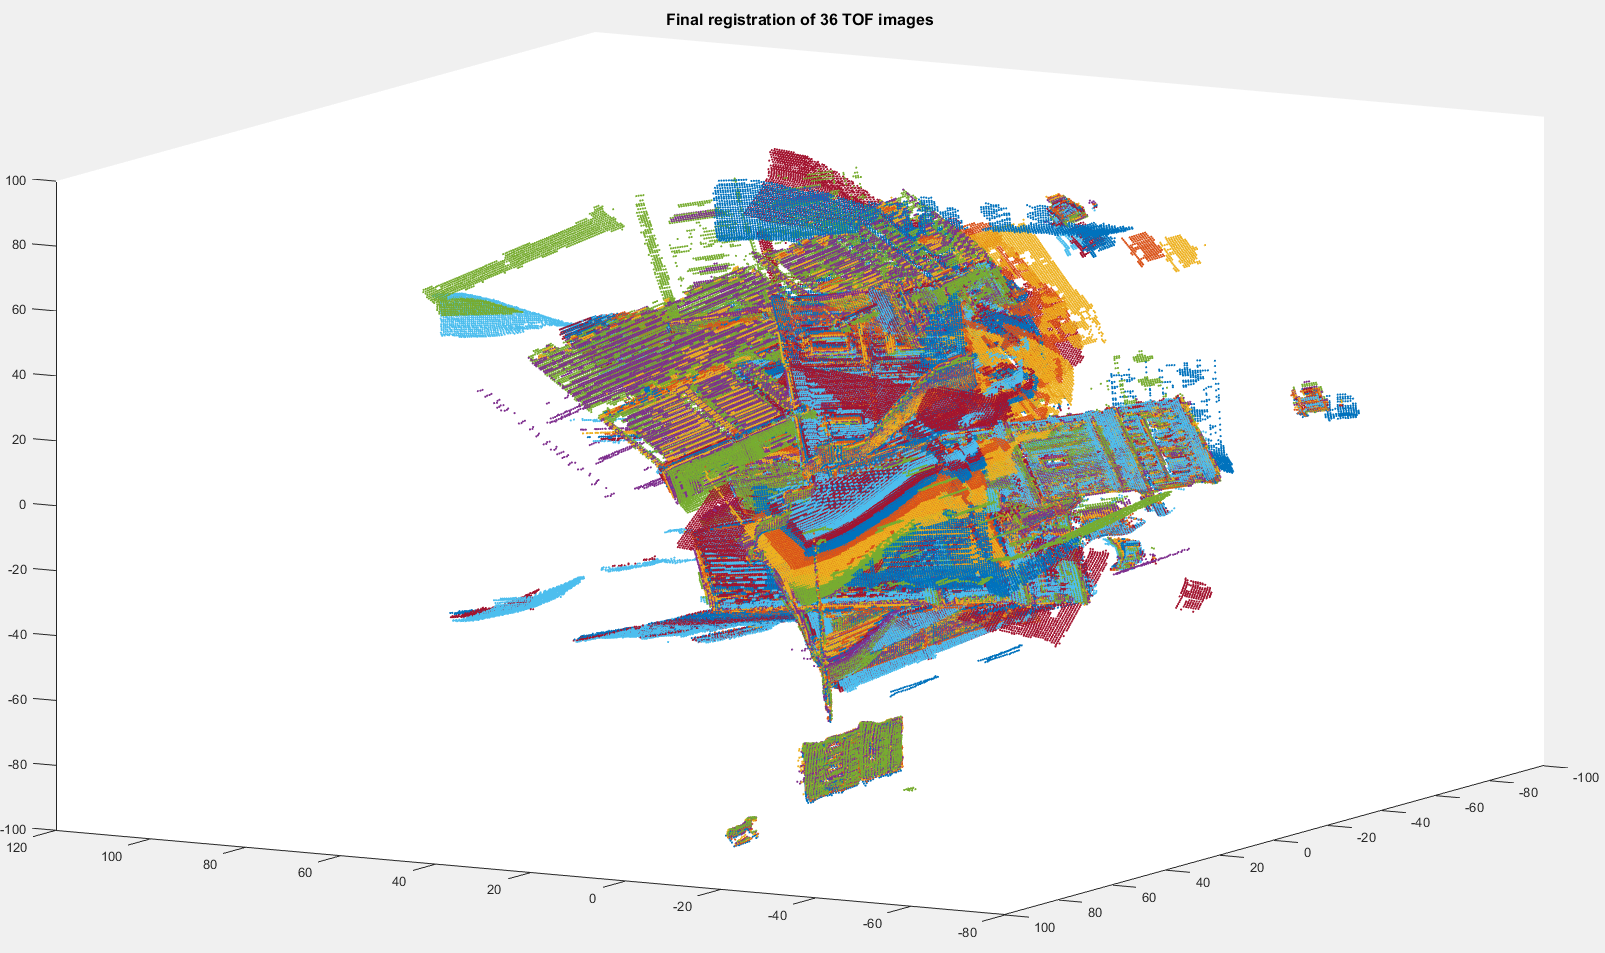
\includegraphics[width=65mm]{figures/JRMPC_result.png}
	\caption{Till vänster: resultat från registrering med ICP. Till höger: resultat från registrering med JR-MPC.}
	\label{fig:icp_vs_jrmpc_result}
\end{figure}

Figur \ref{fig:icp_vs_jrmpc_result} visar resultatet av experimentet. ICP algoritmen har lyckats producera ett resultat som återspeglar kyrkan med några få felaktigheter. JR-MPC däremot har placerat alla punktmoln i varandra på ett sätt som varken liknar punktmolnen innan registrering eller den kyrka som förväntades. I figur \ref{fig:registered_church_serie} ses från övre vänstra till nedre högra bilden delresultatet av 12, 13, 18, 19 samt 20 punktmoln extraherat från en och samma körning av 3DCopy. Notera till exempel resultatet för 20 punktmoln där det tydligt i främre vänstra hörnet på kyrkan syns dubbla hörn. Det här kommer av att punktmolnen som registreras ligger i varandra vid starten. Efter 12 punktmoln behöver därmed nästa moln roteras 130 grader och sannolikheten för ett falskt optimum ökar.
\begin{figure}[H]
	\centering
	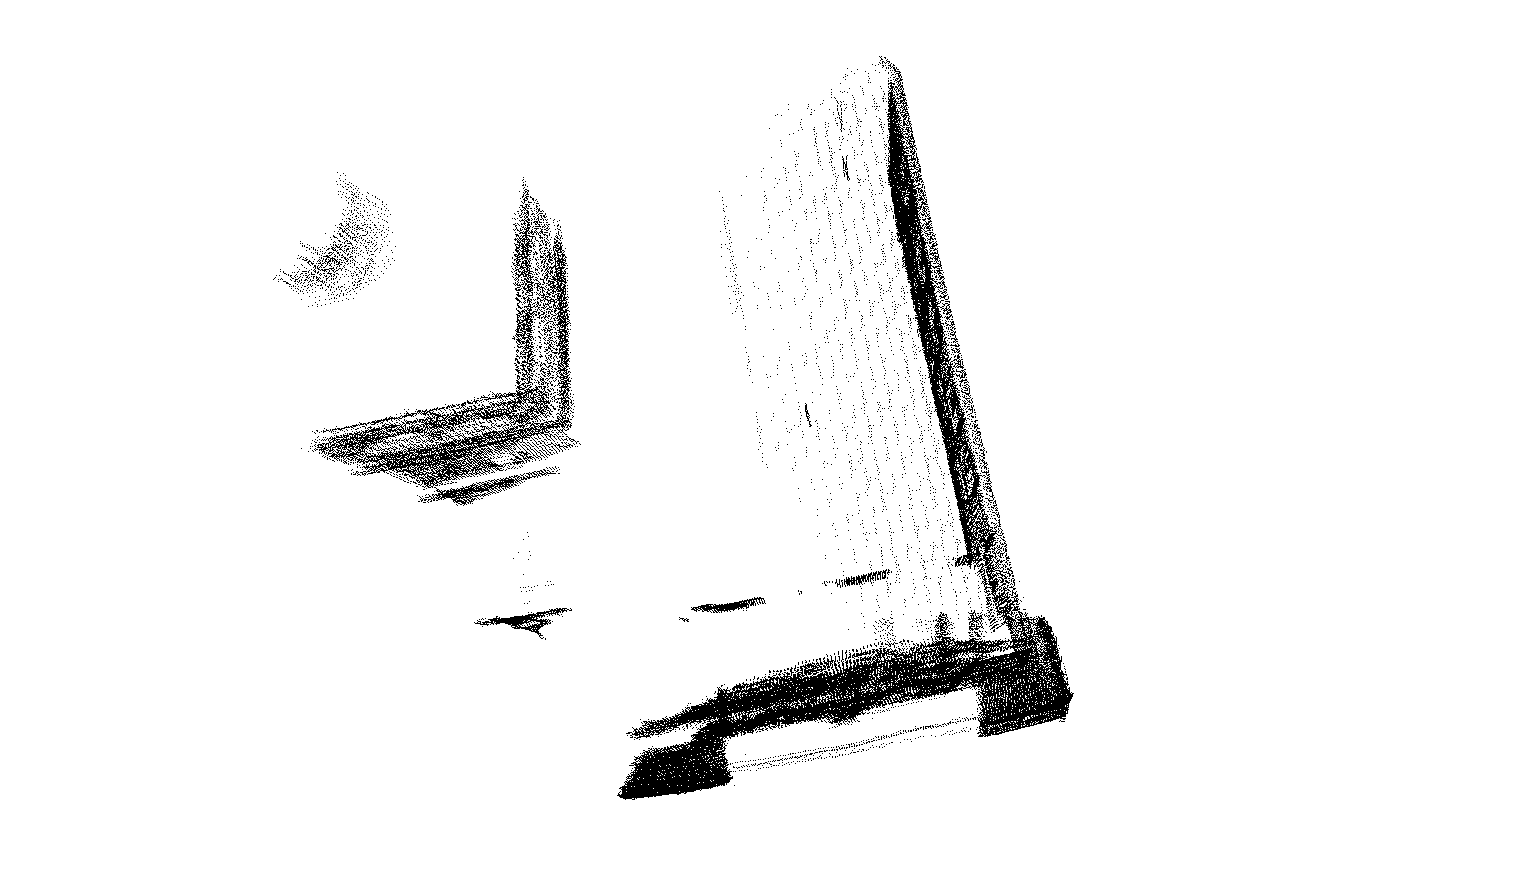
\includegraphics[width=45mm]{figures/12_pc.png}
	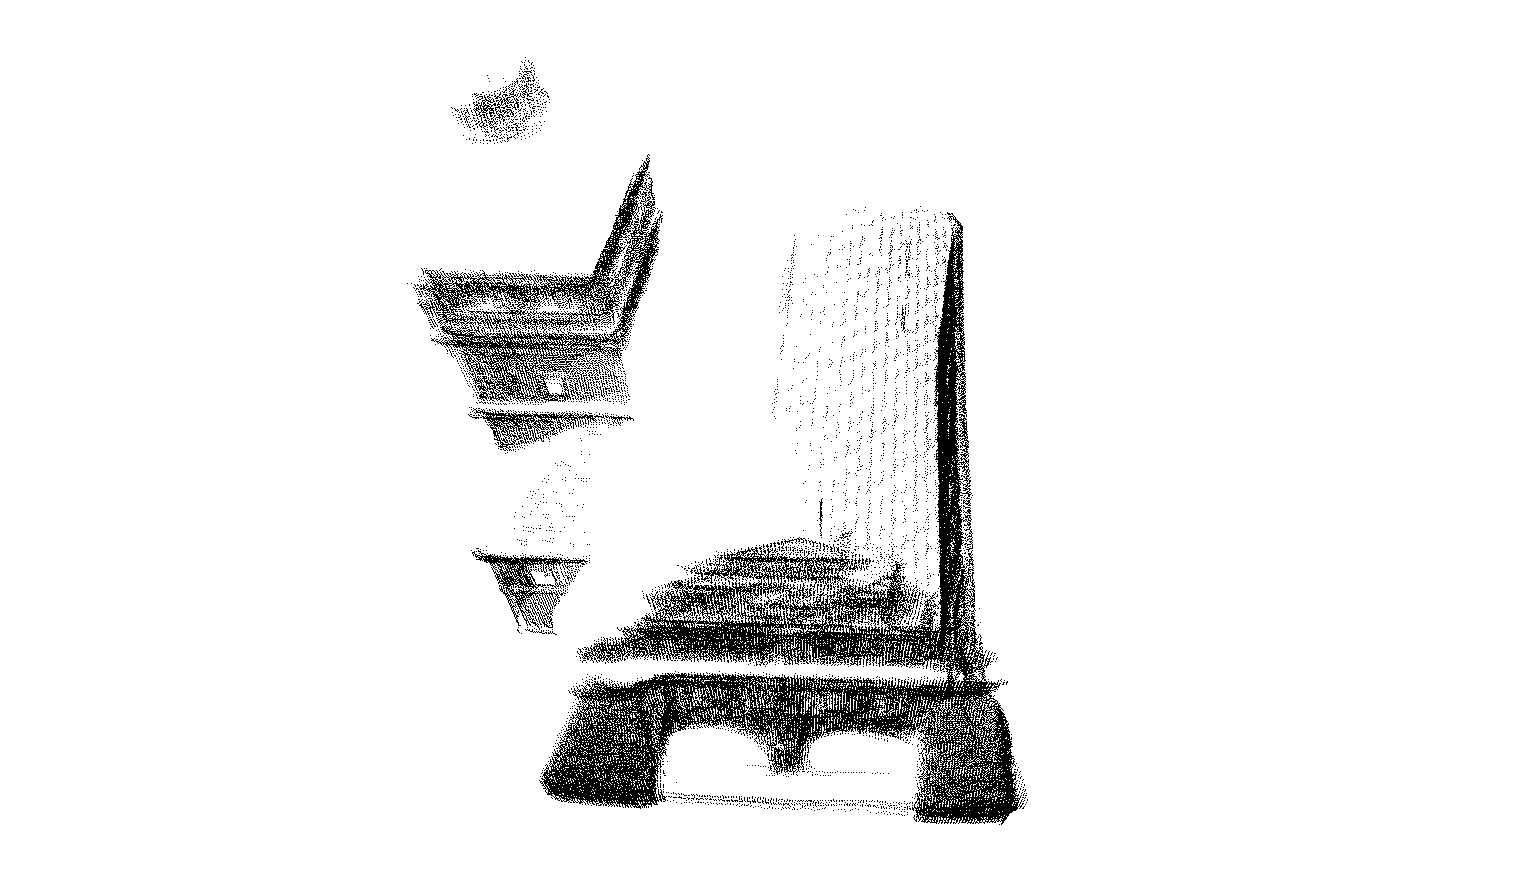
\includegraphics[width=45mm]{figures/13_pc.png}
	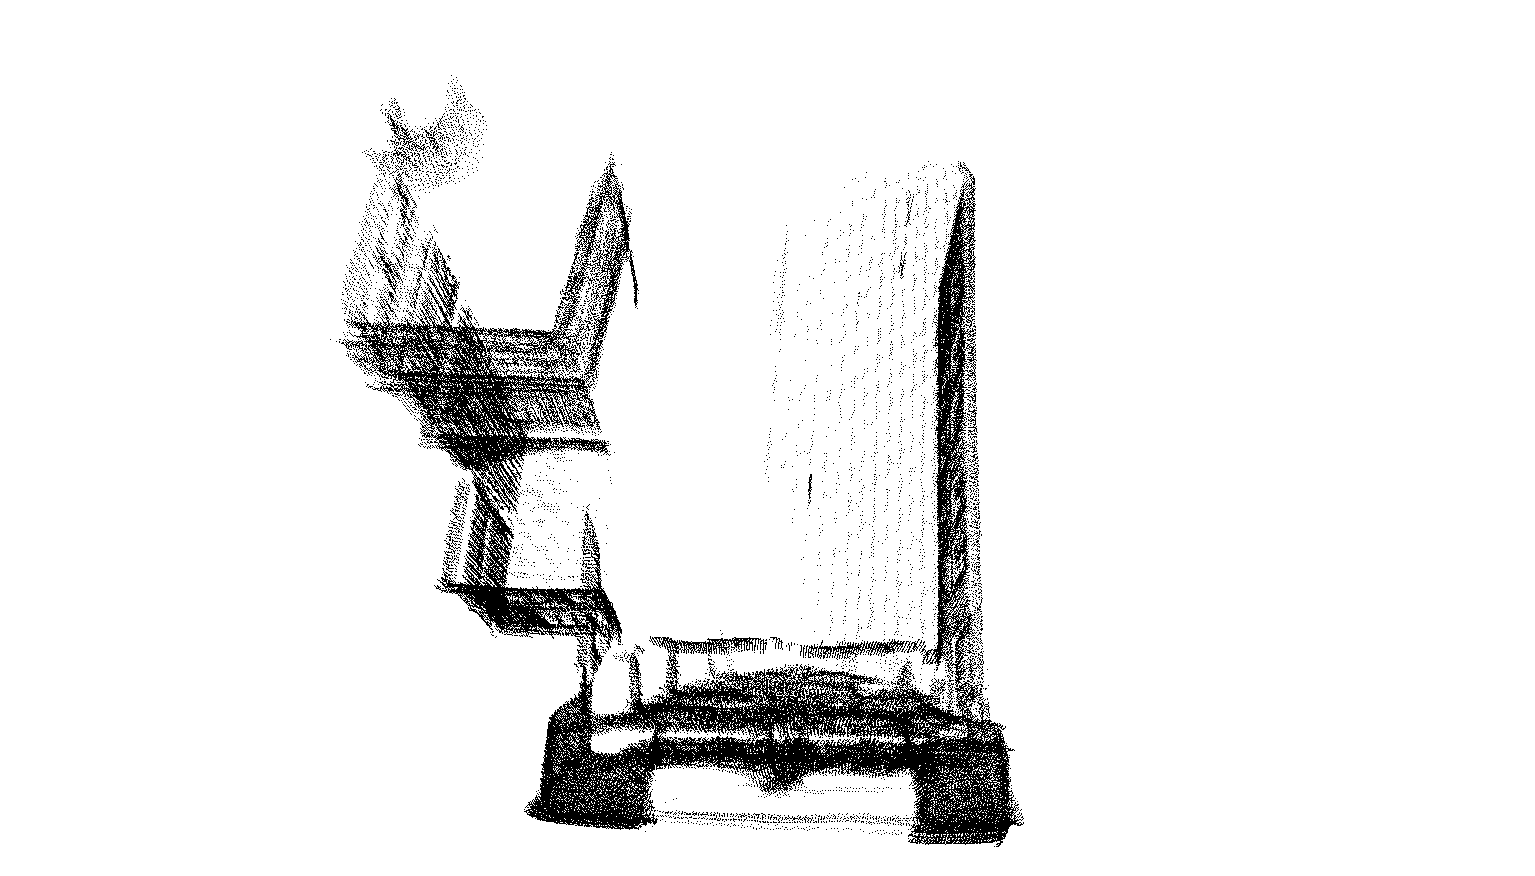
\includegraphics[width=45mm]{figures/18_pc.png}
	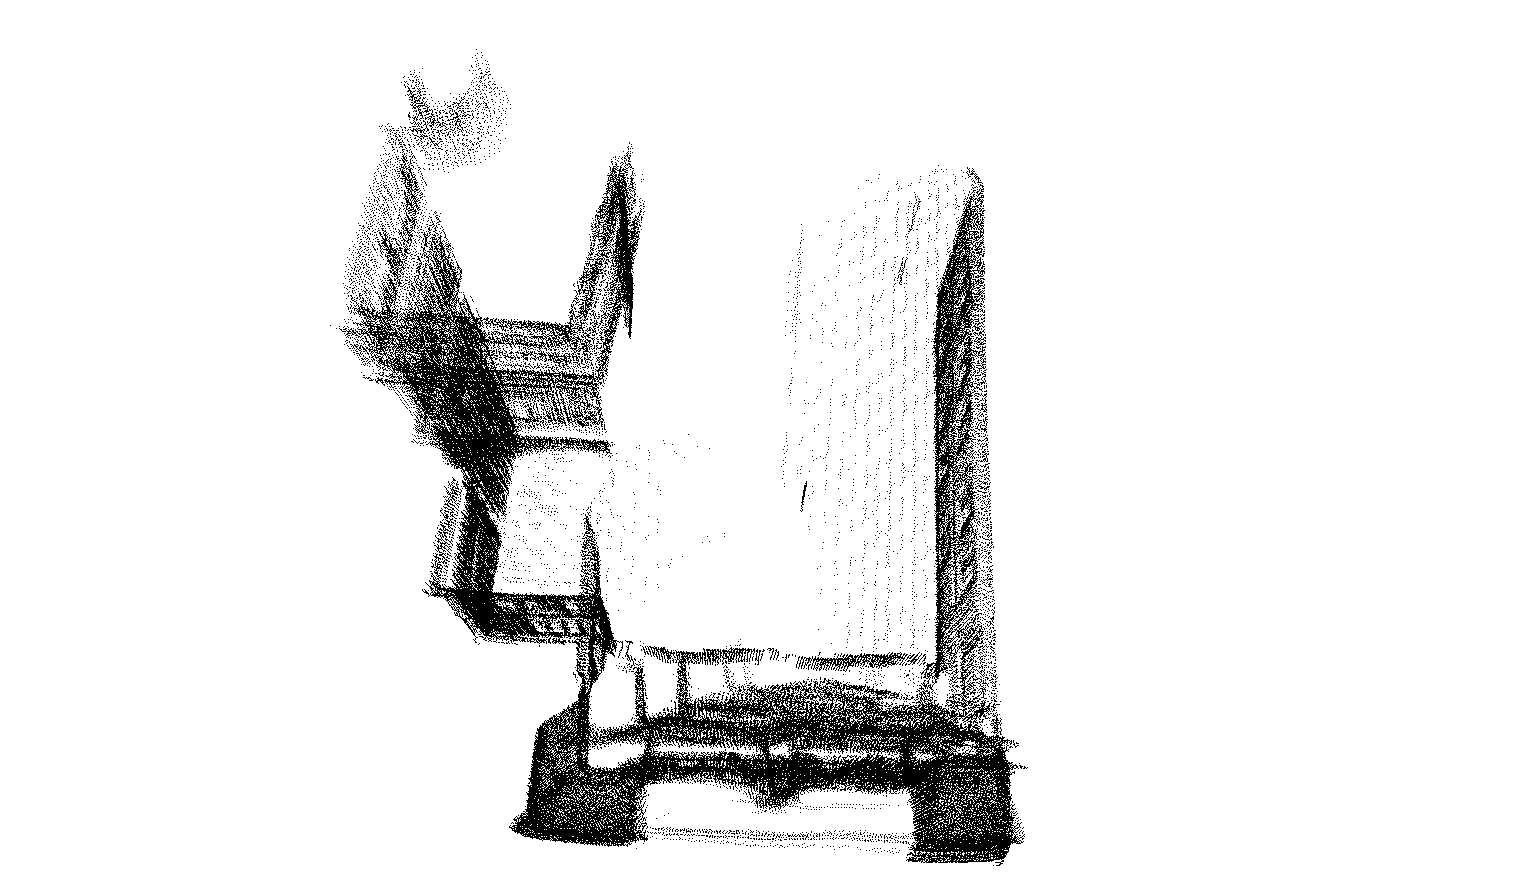
\includegraphics[width=45mm]{figures/19_pc.png}
	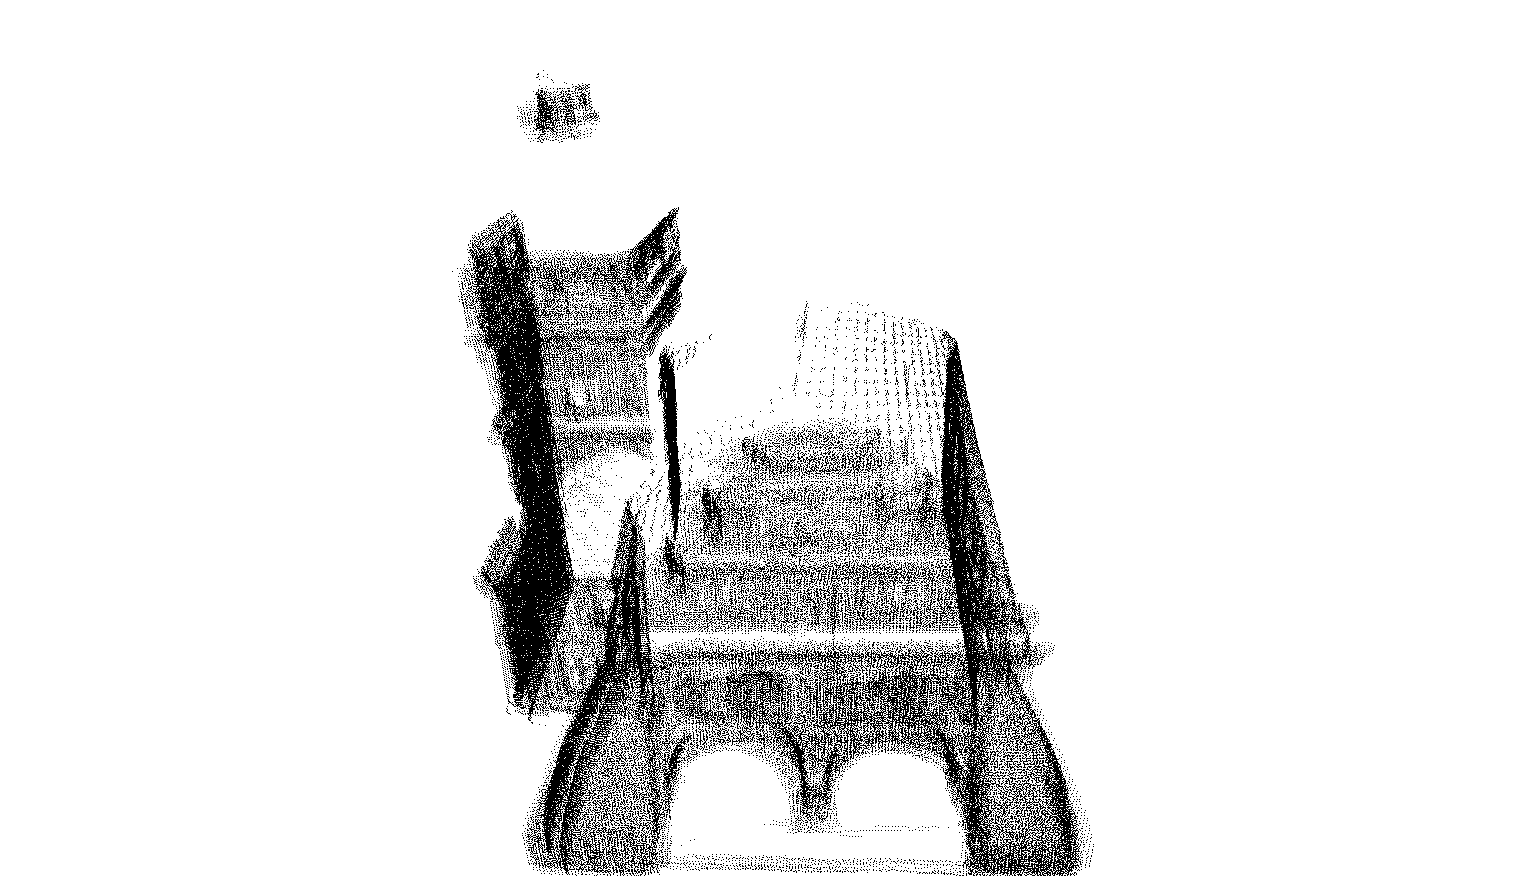
\includegraphics[width=45mm]{figures/20_pc.png}
	\caption{Serie av delresultat från registrering med ICP.}
	\label{fig:registered_church_serie}
\end{figure}

Den poäng (eng. \textit{Fitness score}) som beräknas av ICP visade på att resultatet från de olika körningarna var identiskt. För JR-MPC gjordes en visuell granskning av resultatet och någon skillnad kunde inte identifieras.


\section{Diskussion}
\label{sec:discussion-karlsson}

JR-MPC funkade väldigt dåligt för den typ av data som vi hade. På grund av att algoritmen är väldigt komplicerad och inte ger något delresultat är det svårt att göra några ändringar för att uppnå bättre resultat.

3DCopy använder sig av \textit{Max Iterations}, \textit{Transformation Epsilon} samt \textit{Max correspondence distance}. Då PCLs standardvärden för \textit{RANSAC outlier rejection threshold} samt \textit{Euclidean fitness epsilon} funkade bra för gruppen användes dessa och de kan inte ändras i 3DCopy. Det är dock väldigt lätt att lägga in stöd för det om programmet skulle vidareutvecklas.

\subsection{Metod}

Litteraturstudien som genomfördes som förstudie hade kunnat vara större. Avsaknaden av relevanta källor är något som märkts vid flera tillfällen, både under projektet samt denna rapports framtagande. Man bör dock inte underskatta utvecklingsarbete i utbildningssyfte som var litteraturstudiens primära mål. Då de källor som hittades inte hade mycket överlappande information kunde få jämförelser göras och Evangelidis et al. \cite{Evangelidis-ECCV-2014} fick stå för det mesta av faktan. Dock är det ett publicerat forskningsdokument som funnits tillgängligt under längre tid och som presenterar en bra metod och ett väl dokumenterat tekniskt resultat.

Experimentet gav både bra och identiskt resultat vid varje körning. Det som saknas är en tidsjämförelse men eftersom att resultatet inte är så bra som önskat vid registrering av 36 punktmoln lades tillgängliga resurser på att förbättra resultatet mer än att förkorta körtiden. Efter att experimentet var utfört skapades dock ett filter som filtrerar bort redundant information som både ger bättre resultat, eftersom äldre punktmoln inte får mer och mer vikt under registreringens gång, samt reducerade körtiden signifikant. På grund av tidsbrist kunde dock experimentet inte göras om. 

\subsection{Resultat}

En ordentlig jämförelse mellan algoritmerna som fanns tillgängliga försvårades av att JR-MPC är så matematiskt avancerad. För ordentlig analys uppskattar författaren att det krävs en kandidat i matematik. På grund av detta var det svårt att överhuvudtaget förstå och analysera JR-MPC på samma sätt som gjordes, förhållandevis enkelt, med ICP.


\subsubsection{Experiment}

Experimentet visar att ICP har kommit i närheten av ett bra resultat, se figur \ref{fig:icp_vs_jrmpc_result}. Genom att granska delregistreringen i figur \ref{fig:registered_church_serie} framgår att de första 12 punktmolnen har gått bra att registrera. I delresultatet för 13 punktmoln syns det första punktmolnet som hamnat fel, uppskattningsvis 1-5 grader. Detta fel blir mer och mer tydligt ju fler punktmoln som registreras då alla punktmoln som kommer efter passar bättre med det punktmoln som sitter fel är de tidigare registrerade punktmolnen. 

Första analysen av registreringsresultat resulterade i ett antagande om att ett punktmoln runt nr. 18-20 hade hamnat fel, vilket senare reviderades till resultatet som presenterades här. JR-MPC har däremot helt misslyckats med registreringen som ledde till att projektgruppen helt övergav vidare försök att använda algoritmen. Då JR-MPC saknar delresultat eller tydliga parametrar att ändra är det svårt att analysera vad som orsakar beteendet som syns här.

\section{Slutsatser}
\label{sec:conclusions-karlsson}

Vid digitalt återskapande av fysiska objekt skapas generellt flera punktmoln som ska registreras, dvs sys ihop. För att utföra denna registrering väljs en registreringsalgoritm som är lämpad för uppgiften, framförallt beroende på hur punktmolnen som samlats in ser ut. För ICP handlar det mest om att punktmolnen ska vara någorlunda rätt placerade i ett tänkt gemensamt koordinatsystem. När detta är uppfyllt kan punktmolnen registreras, och förutsatt att man har tillräckligt mycket data kan ett enhetligt punktmoln skapas som representerar det fysiska objektet som skannats.

För gruppens mål funkade ICP bäst men tidiga tester som gjordes gav skäl att undersöka andra algoritmer. Därmed är det svårt att dra någon konkret slutsats om vilken algoritm som är bäst. Det material som tagits fram är inte tillräckligt för att dra en konkret slutsats. Slutsatsen som Bellekens et al. \cite{beller2014modern} kommer fram till, att valet av algoritm är beroende av indata och tillämpning, är dock väldigt rimlig och med mer testdata till grund för deras slutsats är författaren av denna rapport benägen att hålla med.



%%%%%%%%%%%%%%%%%%%%%%%%%%%%%%%%%%%%%%%%%%%%%%%%%%%%%%%%%%%%%%%%%%%%%%
%%% karlsson-report.tex ends here
